\documentclass[a4paper, 12pt, twoside]{scrartcl}
%\usepackage{ngerman}
\usepackage[utf8]{inputenc}
\usepackage{amsmath}
\usepackage{amssymb}
\usepackage{amsfonts}
\usepackage{graphicx}
\setlength{\parindent}{0pt} % No indent at begin of paragraph
\setcounter{secnumdepth}{0} % 0 = No numeration of sections etc.

\title{singlepowder}
\begin{document}
\maketitle

\section{Geometry of the diffractometer}

Figure \ref{fig:goniometer} shows a four circle diffractometer. The angles are shown with the directions used in the program (only $ 2\theta $ is actually used so far). In order to avoid confusion, $ 2\theta $ names the position of the detector while "powder angle" $ \varepsilon $ is used for the angle between the diffracted beam and the direct beam for a certain pixel. The pixel indices $ x $ and $ y $ and the pixel width $ w $ and height $ h $ are shown with the direction used by the classes Geometry and DetectorImage.

The variables in the figure and the following calculation refer to the following variables in the program code:

\begin{align*}
	d &: \text{detector\_distance} & (\mathrm{mm})\\
	2\theta &: \text{twotheta} & (\mathrm{deg})\\
	\varepsilon &: \text{powder\_angle} & (\mathrm{deg})\\
	x &: \text{pixel\_x} & (\mathrm{index})\\
	y &: \text{pixel\_y} & (\mathrm{index})\\
	w &: \text{pixel\_width} & (\mathrm{mm})\\
	h &: \text{pixel\_height} & (\mathrm{mm})\\
	x_c &: \text{centre\_pixel\_x} & (\mathrm{index})\\
	y_c &: \text{centre\_pixel\_y} & (\mathrm{index})\\
	\Delta x &: \text{delta\_x} & (\mathrm{mm})\\
	\Delta y &: \text{delta\_y} & (\mathrm{mm})\\
\end{align*}

\begin{figure}
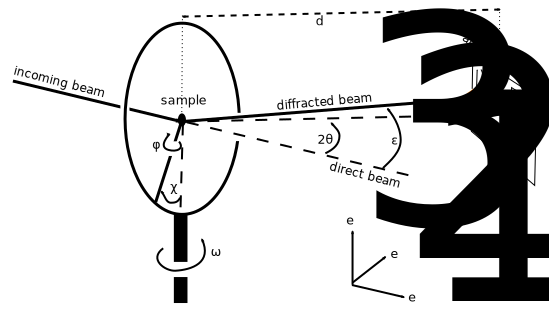
\includegraphics{figs/goniometer.pdf}
\caption{\label{fig:goniometer}Direction of the angles $ 2\theta $, $ \omega $, $ \chi $, $ \varphi $, the pixel indices $ x $, $ y $ and the axes $ e_1, e_2, e_3 $.}
\end{figure}

$ x_c $ and $ y_c $ are the indices of the pixel that is hit by the direct beam when all angles are set to zero. The deviation (in mm) from this pixel is for the pixel with indices $ (x, y) $:

\begin{align*}
	\Delta x &= w(x - x_c) \\
	\Delta y &= h(y - y_c) \\
\end{align*}

Using the basis vectors\footnote{The basis vectors are dimensionless and the coordinates have unit $ \mathrm{mm} $.} defined in Figure \ref{fig:goniometer} (the origin is placed at the pivot point of the goniometer, i.e. the sample), we get for $ 2\theta = 0 $ the following coordinates of the pixel:

\begin{align*}
  \boldsymbol{p} = \begin{pmatrix} d \\ -\Delta x \\ \Delta y \end{pmatrix}	
\end{align*}

The rotation matrix around $ e_3 $ depends on $ 2\theta $:

\begin{align*}
	R = \begin{pmatrix}
		    \cos(2\theta) & -\sin(2\theta) & 0 \\
		    \sin(2\theta) & \cos(2\theta)  & 0 \\
		    0 & 0 & 1
		\end{pmatrix}
\end{align*}

The coordinates of the pixel with indices $ (x, y) $ depend on $ d $ and $ 2\theta $ and are thus:

\begin{align*}
	\boldsymbol{p'} &= R \boldsymbol{p} \\
	 &=
	\begin{pmatrix}
	d \cos(2\theta) + \Delta x \sin(2\theta) \\
	d \sin(2\theta) - \Delta x \cos(2\theta) \\
	\Delta y
	\end{pmatrix}
\end{align*}

The direct beam intersects the detector circle in the following point:

\begin{align*}
	\boldsymbol{r} = \begin{pmatrix} d \\ 0 \\ 0 \end{pmatrix}
\end{align*}

For the angle $ \varepsilon $ between the direct and diffracted beam, the following condition holds:

\begin{align*}
	|\boldsymbol{r}| |\boldsymbol{p}| \cos(\varepsilon) = \boldsymbol{r} \cdot \boldsymbol{p'}~~\mathrm{,}
\end{align*}

where $ \cdot $ denotes the scalar product.

From this, we can calculate the powder\_angle $ \varepsilon $ :

\begin{align*}
	\varepsilon &= \arccos \frac{\boldsymbol{r} \cdot \boldsymbol{p'}}{|\boldsymbol{r}||\boldsymbol{p'}|} \\
	&= \arccos \frac{d ( d\cos(2\theta) + \Delta x \sin(2\theta))}{\sqrt{(d\cos(2\theta) + \Delta x \sin(2\theta))^2 + (d\sin(2\theta) - \Delta x \cos(2\theta))^2}~d} \\
	&= \arccos \frac{d\cos(2\theta) + \Delta x \sin(2\theta)}{\sqrt{(d\cos(2\theta) + \Delta x \sin(2\theta))^2 + (d\sin(2\theta) - \Delta x \cos(2\theta))^2}}
\end{align*}

\end{document}